%----------------------------------------
% Write your notes here
%----------------------------------------

\section{Prediction Vs. Causation}
\textbf{Prediction}: predict future activity for a user from their past data/activity\\
\textbf{Causation}:  agency or efficacy that connects one process (the cause) with another process or state (the effect). But what exactly does causation mean? For example:
\begin{itemize}
  \item What makes an email spam?
  \item How does the stock market works?
  \item Why is Apple, Harry Potter so successful?
\end{itemize}
But there are so many parts, reasons, aspect, possibilities that make one successful. It is almost impossible to figure it out in a scientific sense.

\section{Why is it so hard?}
At any point you have an event, imagine there are so many other things that could have happened. Just by looking at the data, it is not possible to find the root cause. Another more practical way to think about causality: What we can do now and make sense of it? How does one decision have impact on the future? E.g. Should I take this route? How does education actually have impact on your career development?\\
\\
\textbf{Simple Example: What's the effect on your health by going to a hospital?}\\
Let start by looking at people who come to hospital and get treated, and see what’s their health looks like tomorrow. Underlying question: \textit{does hospital cause the change of people’s health tomorrow?}\\
\textit{Think about:} what kinds of people would go to the hospital? People who are less healthy.\\
\textit{Take into account:} Health of the people today really determines whether or not they go the hospital.\\
\textit{What can we do?} Assume sick people go to hospital, and healthy people do not go to the hospital.\\
\textit{If you just look at the data:} going to the hospital, decrease your chance of being healthy.\\
\textit{In reality:} people who go to the hospital are usually sick, and healthy people don't usually go to the hospital.\\
\begin{center} Observed difference =  (Sick and went to hospital -- healthy and stayed home) + (sick if stayed home -- healthy and stayed home)
\end{center}
\noindent\textbf{Key take away: there is, in any kind of data, an inherent bias}
\begin{center} Observed difference =  causal -- bias
\end{center}

\section{Why do we care?}
If you do not know the effect, you cannot make recommendation/decision. We really want to know: If you pick a person, and assume he take this action, what will be the outcome without him actually doing it.
 It is different compared to regression, because in regression get some data, have some outcome you already measured, you just say let me see how many patterns I can find.\\
\\
\textbf{Another example: Xbox user activity}\\
In Regression only want to find out: \textit{how much activity they will produce in the future?}\\
In Causality we care about: \textit{What do we do to increase user activity?}\\
But this can be really complicated:

\begin{figure}[ht]
  \begin{center}
    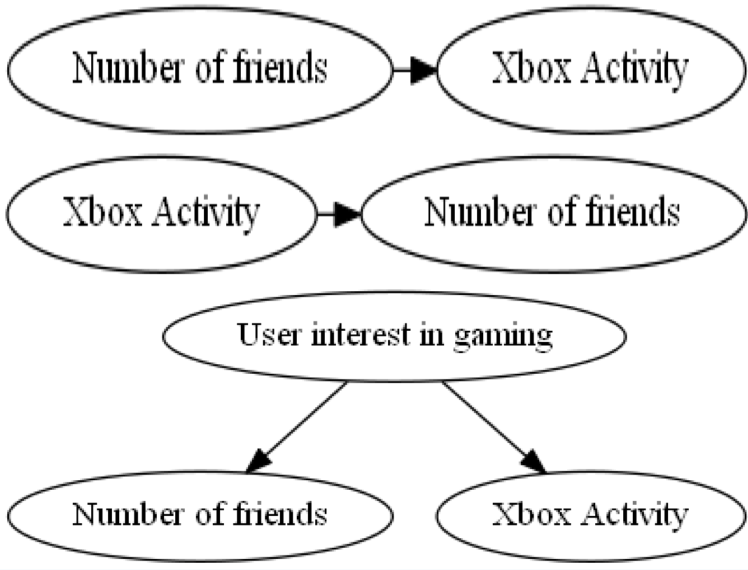
\includegraphics[width=0.5\textwidth]{figures/1.png}
    \caption{
      There can be many causes leading to different outcomes}
    \label{fig:example_figure}
  \end{center}
\end{figure}

\section{Simpson's Paradox (Law?)}
When you have any kind of data, if you don’t condition on the right variables, not only you will get the wrong answer, you will get completely flipped answer.\\
Simplest example: google breast screening test went wrong.\\
\textbf{One Other Example: recommendation engine --- Two algorithms which one is better?}\\
Key Question: how do you know, when you change one algorithm, it works better?\\
Let’s look at the data. Random 1000 session for each algorithm. Measure Click Through Rate (CTR).\\
\begin{figure}[ht]
  \begin{center}
    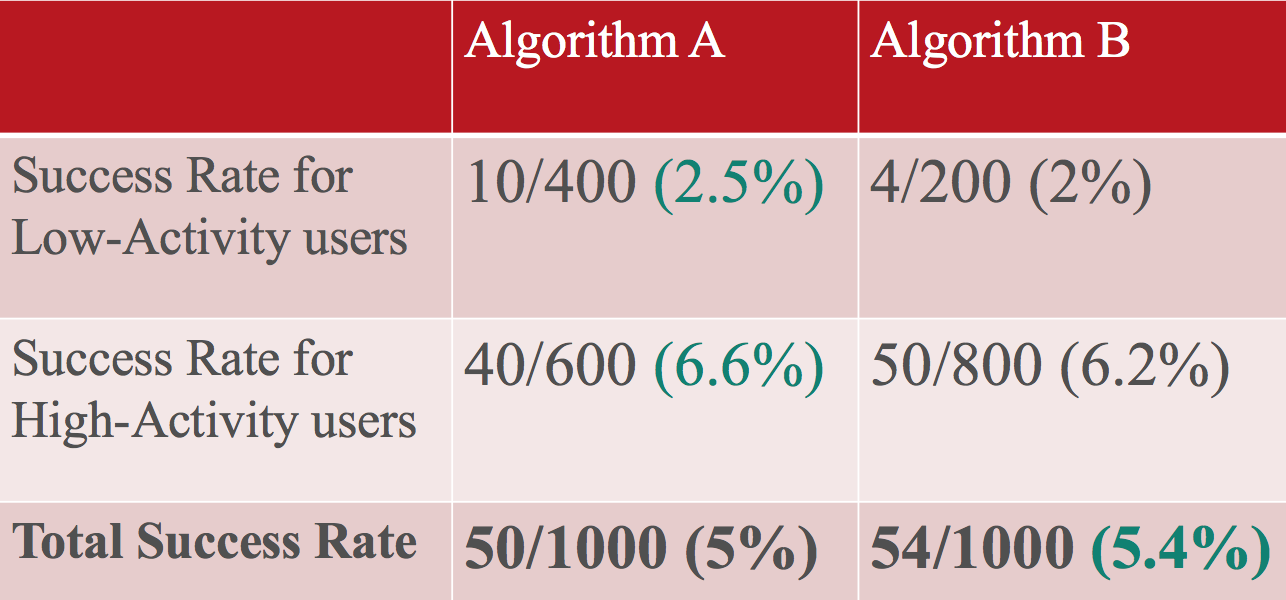
\includegraphics[width=0.5\textwidth]{figures/2.png}
    \caption{
      Is Algorithm A better?}
    \label{fig:example_figure}
  \end{center}
\end{figure} \\

\noindent Answer: As usual, may be, may be not.\\
A different control variable gives the same data a very different outcome\\
\begin{itemize}
  \item Different kinds of user (low/high activity user)
  \item Time of day
  \item Sample size
\end{itemize}

\noindent Stratification --- this thing we changes will have different effects on different groups, so we will break everything into different groups, and within each group we will do experiment, and look effects within each stratum. Picking which group we are going to do beforehand. You want to stratify a lot of things, Fixing different variables, getting exponential number of cases.\\

\section{How do we solve Simpson's Paradox?}
Let's go back to the hospital example: \\
\textit{What we wanna do:} take the world, make a clone of it (parallel universe) and one case bring this guy to the hospital, and one case we don’t. Everything else is the same, everything is identical except the change. We know nothing could affect the treatment outcome, other than the one thing that we changed. (Idea of counter-factual, but we can’t observe it)\\
\textit{In reality:} can’t make copies of the universe. Instead, for each person we are interested, we will flip a coin, and tell them whether they go to the hospital or not going to the hospital. Treatment vs. control. Most important thing here, is that we are flipping the coin. (even if someone’s healthy, we are going to send him to the hospital; some one’s sick don’t send them to hospital)\\
\textit{Key point:} randomly send people to hospital or make them stay home. Reason: The reason they go to hospital is nothing but the result of coin flip, this produces a controlled situation. (similar to the idea of parallel universe) \textbf{Key Recipe: TRUE RANDOMNIZATION}\\
When we are flipping the coin (creating world A, world B), we are taking away the relationship any reason that people might have chosen to be in the treatment, with all the other condition they had before.\\ \textbf{MAKING SELECTION BIAS ZERO.}
\begin{center}
CAUSAL EFFECT = OBSERVED DIFFERENCE
\end{center}
\textbf{A|B TESTING}: (sometimes called split testing) a randomized experiment with two variants, A and B, which are the control and variation in the controlled experiment. It is much easier to measure causal effect. The bigger size the experiment you run, greater statistical power, more able to identify cause. However, in reality it is very hard to create an equal world 1 and world 2.\\
\textit{Many challenges and difficulties:} 
\begin{itemize}
  \item \textbf{Experimenter effect:} if people know they are in an experiment, they will change the outcome.
  \item Difficult to create convincing world: when we actually flip a coin, people in two groups are the same.
\end{itemize}

\section{Internal and External Validity Trade-off}
\textbf{Internal validity}: experiment is RIGHT, anything but the coin flips we did change the outcome\\
e.g. ethical dilemma in the hospital\\
\textbf{External Validity:} validity to generalize, take this experiment, apply it to practice, does the result carry over? \\
e.g. if we decide to sell this drug on market, will it be as effective as it were in the experiment? Maybe clinical trials, we rigorously monitor patients, but in practice does not adhere.\\
\textbf{Internal:} could anything other than the treatment have produced this outcome?\\
\textbf{External:} do the results of the experiment hold in settings we care about?
\\
\textbf{How social science experiments are done?}\\
\begin{enumerate}
  \item Lab Experiment: held at university, bring people in, make them do experiment, measure the result.
  	\begin{enumerate}
  	\item High degree of procedural control
  	\item Optimized for causal inference
  	\item Artificial environment
    \item Simple tasks, demand effects
    \item Homogeneous WEIRD* subject pools (Western, educated, industrialized, rich, democratic countries)
    \item Time/scale limitations
	\end{enumerate}
  \item Field Experiment:go to real world organization, having people flipping coins, doing experiments
  	\begin{enumerate}
  	\item High degree of procedural control
  	\item Optimized for causal inference
  	\item Fewer constraints on location
    \item Longer periods of time
    \item More samples of data
    \item More effort
    \end{enumerate}
\end{enumerate}

You are choosing between complexity (more precise control) vs. realism (more generalizable)

\section{Natural Experiments}
What can you do if you don’t have experiments? Not much, you can try a few strategy
Even today we don’t know if we can not do experiments. What is something you can exploit? Understand problem, understand data, understand what you can exploit.\\

\textbf{1) find experiment in nature, as-if random}\\

\begin{figure}[ht]
  \begin{center}
    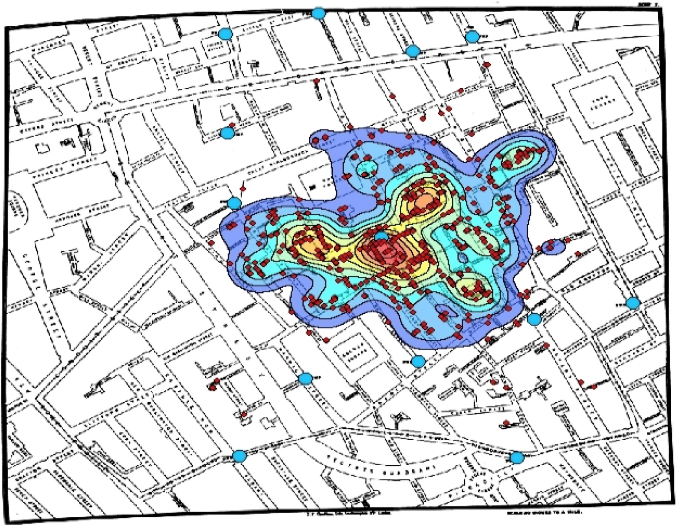
\includegraphics[width=0.5\textwidth]{figures/3.png}
    \caption{
      1854: London was having a devastating cholera outbreak}
    \label{fig:example_figure}
  \end{center}
\end{figure} 
\noindent Example: Jon Snow and his Maps.
But if you think about it: that just shows people who live near the pond got sick, maybe people who live by pond got bad habits, bad neighborhood, air by the pond is bad.\\
2nd thing Jon Snow did: he showed there is as-if random. There are two companies, one getting water downstream (contaminated), one getting water upstream(uncontaminated), by just looking at some person who went to first/second company) Have sufficient evidence to convince yourself and others that this difference could have not happened without the corresponding changes 
(TREATMENT AND CONTROL)
\begin{figure}[ht]
  \begin{center}
    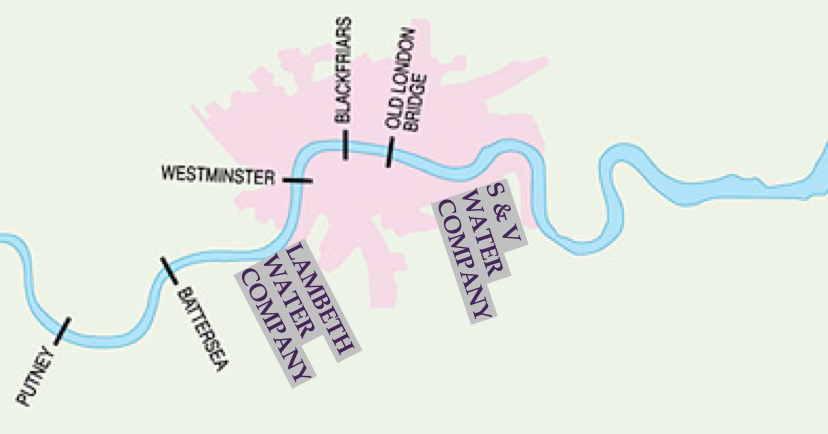
\includegraphics[width=0.5\textwidth]{figures/4.png}
    \caption{
      Two major water companies for London: one upstream and one downstream.}
    \label{fig:example_figure}
  \end{center}
\end{figure} 

\noindent Why was Snow’s study so convincing?\\
\begin{itemize}
  \item Choice of water company cannot cause cholera. 
  \item Choice of water company was not related to people’s neighborhood or its air quality.
\end{itemize}

\textbf{2) Instrumental variables}\\
You don’t change water (root cause) itself, you do something else that is instrumentally changing where people are having their water from. Change the distribution of the cause.\\
e.g. lottery system how military service affect future earnings
When veterans come back, will they be a good earner? People can make all kinds of decisions, once we know the lottery is random, if that’s true. 
"An important question in economics research is what determines earnings. Angrist (1990) evaluated the effects of military service on lifetime earnings. Using statistical methods developed in econometrics, Angrist capitalized on the approximate random assignment of the Vietnam War draft lottery, and used it as an instrumental variable associated with eligibility (or non-eligibility) for military service. Because many factors might predict whether someone serves in the military, the draft lottery frames a natural experiment whereby those drafted into the military can be compared against those not drafted because the two groups should not differ substantially prior to military service. Angrist found that the earnings of veterans were, on average, about 15 percent less than the earnings of non-veterans." (From WikiPedia)\\

\textbf{3) Regression discontinuities:}\\
Regression discontinuity design (RDD)is a quasi-experimental pretest-post test design that elicits the causal effects of interventions by assigning a cutoff or threshold above or below which an intervention is assigned. By comparing observations lying closely on either side of the threshold, it is possible to estimate the average treatment effect in environments in which randomization is unfeasible



